% event stuff

A series of selection cuts are applied to data and Monte-Carlo samples to obtain a high-purity sample of \Wboson\ event candidates. Following a summary table, this chapter explains the motivation behind some of the cuts, describes the selection efficiency in data and Monte-Carlo, and shows the kinematic distributions of selected events.

\section{Summary of Selection}
\label{sec:event:fullsel}

\begin{itemize}
\item Veto events not in the Good Run List (data only).
\item Reject events suffering from noise burst with \verb|larError| $> 1$.
\item Require the first reconstructed primary vertex in the collection to have $\ge 3$ associated tracks.
\item Events must be triggered by the single muon trigger.
\item Events are required to have one reconstructed muon, passing the following cuts:
  \begin{itemize}
  \item Combined STACO muon
  \item Track quality criteria
  \item $\abseta < 2.4$
  \item $\pt > 25\gev$ ($\pt > 20\gev$ for double-differential measurement)
  \item Track isolation
  \end{itemize}
\item Reject events with $> 1$ muon passing the above cuts.
\item The recommended \MET\ cleaning cuts are applied.
\item Veto events with a jet in a LAr hole.
\item $\met > 25\gev$.
\item $\mt = \sqrt{2 p_{T,\ell} \met \cdot (1 - \cos{\Delta\phi (\ell,
      \met) )}}> 40\gev$.
\end{itemize}

\subsection{Good Run List}
Events in luminosity blocks that suffered from severe detector defects (such as a non-operating calorimeter) are excluded from the very beginning. This cut is only applied in data because Monte-Carlo does not simulate these defects.

%https://twiki.cern.ch/twiki/bin/viewauth/AtlasProtected/LArCleaningAndObjectQuality
\subsection{LAr Error}
The liquid argon calorimeter suffers from rare noise bursts and data integrity problems during readout. These conditions may bias the \met\ estimation, so the affected events are flagged and removed from the data.
 
\subsection{Primary Vertex}
The primary vertex with the highest scalar sum-$p_T$ of the tracks pointing to the vertex is required to have at least 3 tracks to ensure that it is reconstructed correctly. Good knowledge of the primary vertex is necessary for muon and jet reconstruction algorithms.

\subsection{Trigger}
The event is required to satisfy the EF\_mu18 or EF\_mu18\_medium triggers, as described in Sec.~\ref{sec:event:trig}. The Muid family of trigger was chosen over the alternative MuGirl chains due to $\eta$-asymmetric problems in the MuGirl trigger (see Appendix~\ref{appendix:ac}).

\subsection{Track Quality Criteria}
\label{subsec:TrackQuality}
Inner detector tracks associated with combined muons are required to satisfy a series of hit-level requirements to ensure good quality of the helix parameters and reduce fakes:

\begin{itemize}
\item If hits in the inner pixel layer are geometrically expected, then the muon track must have at least 
one inner pixel layer hit;
\item $N_{PIX}+N_{DEAD-PIX} >$ 1, where $N_{PIX}$ is the number of pixel hits and $N_{DEAD-PIX}$
      is the number of crossed dead pixel sensors;
\item $N_{SCT}+N_{DEAD-SCT} \ge$ 6, where $N_{SCT}$ is the number of SCT hits and $N_{DEAD-SCT}$
      is the number of crossed dead SCT sensors;
\item $N_{DEAD-PIX}+N_{DEAD-SCT} <$ 2;
\item A successful TRT extension is required in the eta acceptance of the TRT. 
If $N_{TRT-HITS}$ denote the number of TRT hits on the muon track, $N_{TRT-OUTLIERS}$ the number of 
TRT outliers on the muon track (hits that are away from any nearby tracks, or those that failed to form a smooth trajectory with a nearby Pixel+SCT track), and $N_{TRT} = N_{TRT-HITS}+N_{TRT-OUTLIERS}$, then
\begin{itemize}
\item in the interval $|\eta| <$ 1.9: $N_{TRT} >$ 5 and $N_{TRT-OUTLIERS}$/$N_{TRT} <$ 0.9 are required;
\item in the interval $|\eta| >$ 1.9: if $N_{TRT} >$ 5 then $N_{TRT-OUTLIERS}$/$N_{TRT} <$ 0.9 is 
required; if $N_{TRT} \le$ 5, the muon is accepted regardless of the number of outliers.
\end{itemize}
\end{itemize}

In addition, the muon track must point to within 10 mm of the primary vertex ($|z_{\mu}-z_{PV}| <$ 10 mm) to suppress cosmic rays.

\subsection{Muon Isolation}
\label{subsec:MuonIsolation}
Muons produced in \Wmn\ decays are expected to be isolated from nearby tracks, in contrast to muons produced in heavy-flavor decays and in-flight decays of kaons. This difference is exploited through a relative tracking isolation cut: the $p_T$-sum of all tracks within a cone of $\Delta R = 0.4$ around the muon (excluding the muon itself) is divided by the muon $p_T$, resulting in a dimensionless quantity that peaks at 0 for well-isolated muons.
\begin{equation}
I_\mu = \frac{p_T^\mathrm{cone40}}{p_T^{\mu}} < 0.1
\end{equation}\label{eq:isolation}

The difference in the relative isolation distributions for heavy-flavor QCD Monte-Carlo and \Wmn\ Monte-Carlo is illustrated in Fig.~\ref{fig:event:isoplot}.

\begin{figure}[htb]
  \begin{center}
    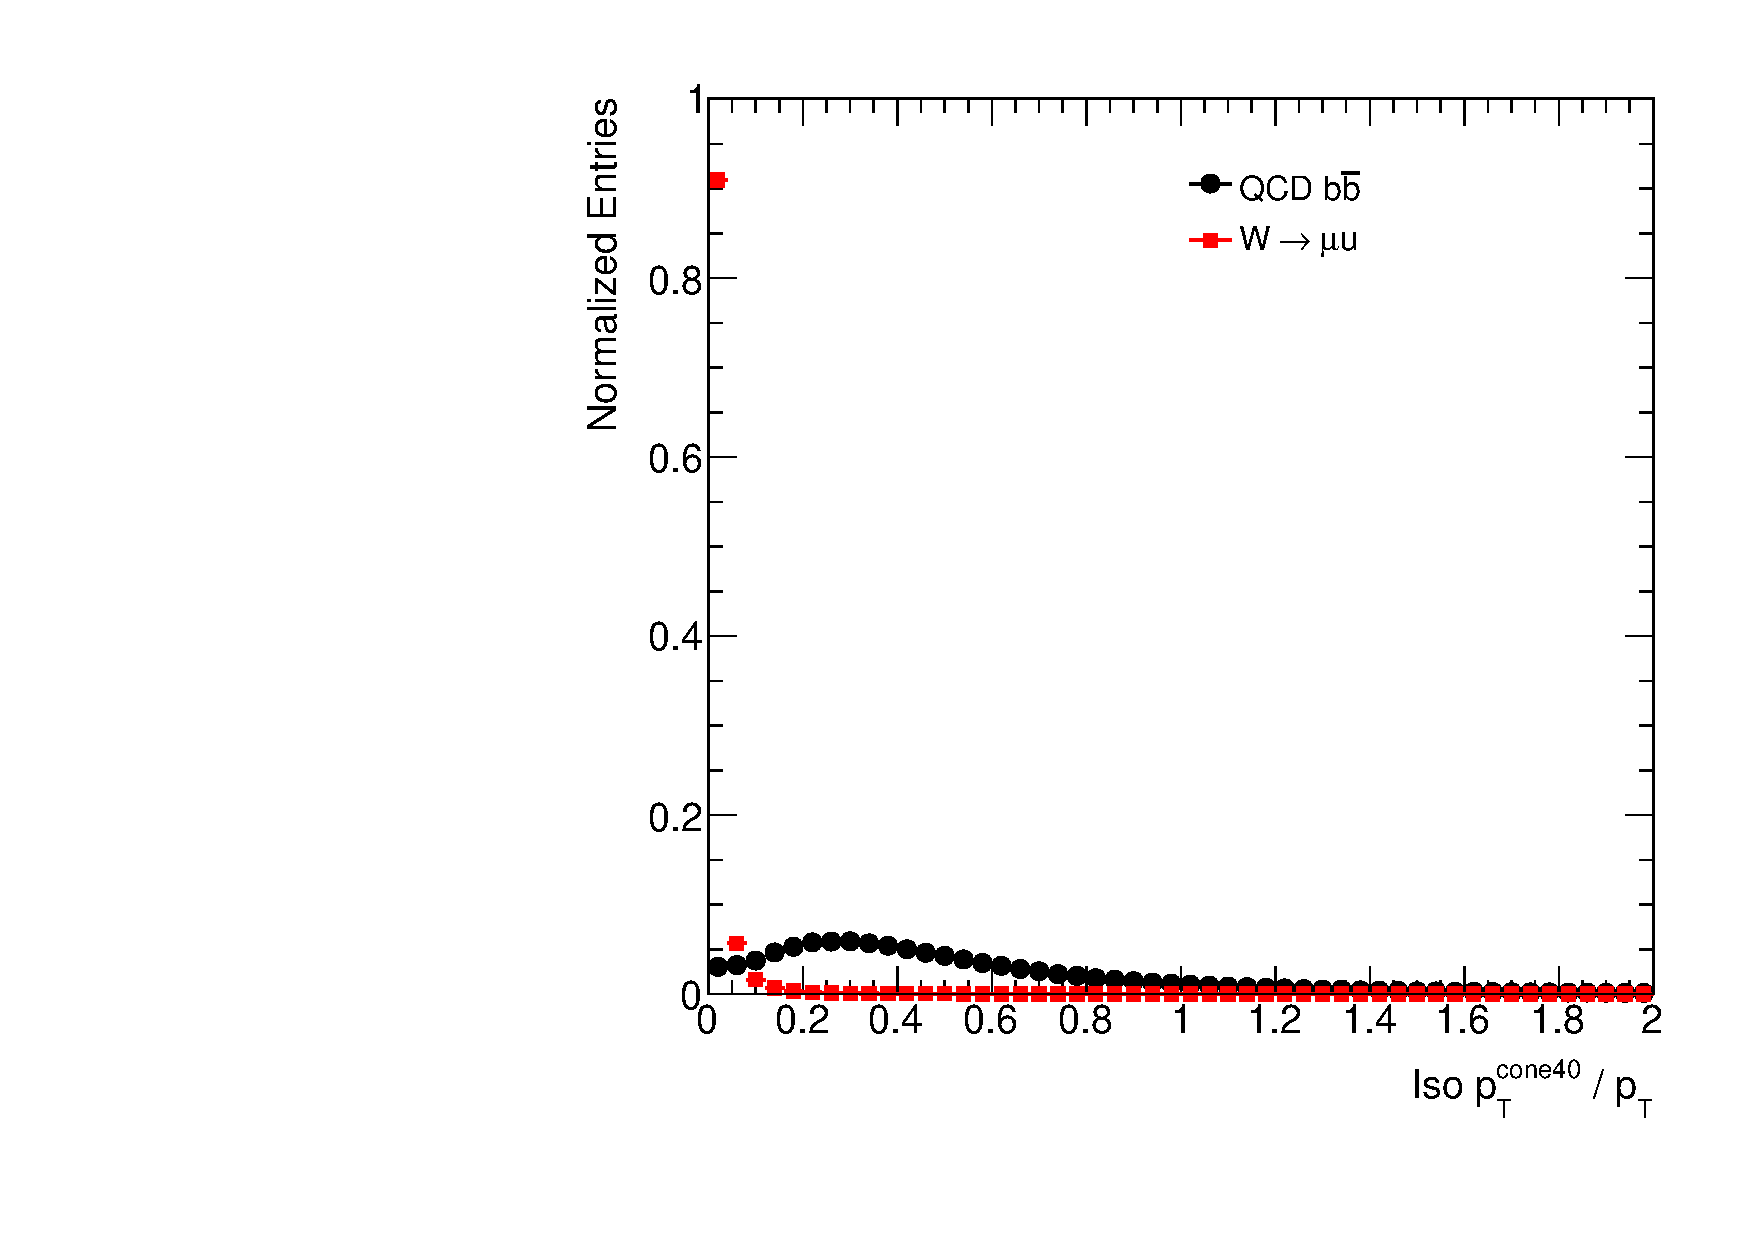
\includegraphics[width=0.7\textwidth]{event/fig/TEST_ISOPLOT_NEG_lepton_ptiso40r}
    \caption{Relative isolation $p_T^{cone40}/{p_T}$ for the signal (\Wmn) and heavy-flavor QCD Monte-Carlo ($b\overline{b} \rightarrow \mu$). The distributions are normalized to the same area}
    \label{fig:event:isoplot}
  \end{center}
\end{figure}

\subsection{Second Muon Veto}
Events with additional muons are rejected to minimize the \Zmm\ background.

\subsection{\met\ Cleaning}
Events containing a jet pointing to misbehaving section of the calorimeter are vetoed to avoid biasing \met\ reconstruction.

\subsection{LAr Hole Veto}
In late April of 2011, 6 front-end boards of the liquid argon calorimeter failed, resulting in a well-defined acceptance hole. Events with jets pointing in the overall direction of the LAr hole are rejected to avoid biasing \met.

\subsection{\met\ and $m_T$ cuts}
Missing transverse energy and W transverse mass cuts consistent with a \Wmn\ decay are applied to reject background events and make the experimental measurement in a phase space similar to that used at the generator level (Sec.~\ref{method:fid:space}).

\section{Selected Events in Data and MC}

\subsection{Cutflows}

\paragraph{Data}

The numbers of candidate events after the different selection cuts are given in Table \ref{tab:Wmunu:cutflow_data_pt25}.

\paragraph{Simulation}

The numbers of selected events after the different selection cuts are given in Tables \ref{tab:Wmunu:cutflow_mc_POS_pt25} ($W^{+} \rightarrow \mu^{+} \nu$) and \ref{tab:Wmunu:cutflow_mc_NEG_pt25} ($W^{-} \rightarrow \mu^{-} \nu$), using the nominal signal Monte-Carlo and applying all re-weightings and scale-factors. These tables reflect the actual Monte-Carlo statistics - in other words, the numbers have not been scaled to the integrated luminosity in the data.

\begin{table}
\begin{center}
\input{Wmunu/figures/cutflow/data_pt25}
\caption{ Cutflow for \Wmn\ candidate events in data ($p_T~>~25~\GeV$). Data events that don't have at least one 8 \GeV muon (of any kind) were dropped at the ntuple creation stage.}
\label{tab:Wmunu:cutflow_data_pt25}
\end{center}
\end{table}


\begin{table}
\begin{center}
\input{Wmunu/figures/cutflow/mc_POS_pt25}
\caption{ Cutflow for $W^{+} \rightarrow \mu^{+} \nu$ events in the nominal Monte Carlo signal sample~(Powheg+Pythia). Pileup, vertex position, and $p_T^{W}$  weights are applied, but the counts are not scaled to the integrated luminosity in the data. The number of selected events after the application of efficiency scale factors is shown in the last row. Note that the Monte-Carlo events are not restricted to a fiducial region at truth level, so the reported efficiencies are a mixture of acceptance and reconstruction efficiency factors. }
\label{tab:Wmunu:cutflow_mc_POS_pt25}
\end{center}
\end{table}


\begin{table}
\begin{center}
\input{Wmunu/figures/cutflow/mc_NEG_pt25}
\caption{ Cutflow for $W^{-} \rightarrow \mu^{-} \nu$ events in the nominal Monte Carlo signal sample~(Powheg+Pythia). Pileup, vertex position, and $p_T^{W}$  weights are applied, but the counts are not scaled to the integrated luminosity in the data. The number of selected events after the application of efficiency scale factors is shown in the last row. Note that the Monte-Carlo events are not restricted to a fiducial region at truth level, so the reported efficiencies are a mixture of acceptance and reconstruction efficiency factors.}
\label{tab:Wmunu:cutflow_mc_NEG_pt25}
\end{center}
\end{table}

\subsection{Kinematic distributions}
Kinematic distributions of the selected \Wmn\ candidate events are shown in Figs.~\ref{fig:Wmunu:mu_angle25}, \ref{fig:Wmunu:mu_kine25} and~\ref{fig:Wmunu:mt_pt25}. The muon $p_{T}$ cut is set to 25 \GeV. The normalizations for QCD predictions are obtained from a template fit to the $E_T^{Miss}$ distribution in the inclusive $\eta - p_{T}$ region, repeated separately for each systematic variation. The fits are performed as described in Sec.~\ref{sec:wmnu:qcdbkg}. The final Monte-Carlo histograms are normalized to data. This is also done separately for each systematic in order to accentuate the differences in shapes introduced by the systematic variations, rather than differences in overall normalization, which are dominated by the cross-section and PDF uncertainties.

For all plotted distributions, Monte-Carlo predictions agree with the data within their uncertainty bands. The large systematic uncertainty in the tails of \MET\ (Fig.~\ref{fig:Wmunu:mu_kine25}), \Wboson\ $m_T$ and \Wboson\ $p_T$ (Fig.~\ref{fig:Wmunu:mt_pt25}) distributions are largely correlated and are driven by the use of alternative Monte-Carlo generators, as described in Sec.~\ref{sec:sys:theoryunc}.

% Selected control plots in slices of muon $p_{T}$ are available in Appendix~\ref{sec:Wmunu:AppendixControlPtBins}
\begin{figure}[phtb]
  \begin{center}
        \subfigure[$\eta$ : $\mu^+$]{%
          \includegraphics[width=0.45\textwidth]{Wmunu/figures/control_plots/inclusive25/P_stack_d3_eta_lpt_met_y_2__1_z_0__1_POS}
        } 
       \subfigure[$\eta$ : $\mu^-$]{%
         \includegraphics[width=0.45\textwidth]{Wmunu/figures/control_plots/inclusive25/P_stack_d3_eta_lpt_met_y_2__1_z_0__1_NEG}
        } \\
 \caption{ Distributions of the muon $\eta$ for selected \Wmunup~(left) and \Wmunum~(right) events. }
 \label{fig:Wmunu:mu_angle25}
 \end{center}
\end{figure}

\begin{figure}[phtb]
  \begin{center}
        \subfigure[$p_T$ : $\mu^+$]{%
          \includegraphics[width=0.45\textwidth]{Wmunu/figures/control_plots/inclusive25/P_stack_lpt_POS}
        } 
       \subfigure[$p_T$ : $\mu^-$]{%
         \includegraphics[width=0.45\textwidth]{Wmunu/figures/control_plots/inclusive25/P_stack_lpt_NEG}
        } \\
        \subfigure[$E_T^{Miss}$ : $W^{+}$]{%
          \includegraphics[width=0.45\textwidth]{Wmunu/figures/control_plots/inclusive25/P_stack_d3_abseta_lpt_met_x_0__1_y_2__1_POS}
        } 
       \subfigure[$E_T^{Miss}$ : $W^-$]{%
         \includegraphics[width=0.45\textwidth]{Wmunu/figures/control_plots/inclusive25/P_stack_d3_abseta_lpt_met_x_0__1_y_2__1_NEG}
        } \\
 \caption{ Distributions of the muon $p_{T}$ (top) and missing transverse energy (bottom) for selected \Wmunup~(left) and \Wmunum~(right) events ($p_{T}~>~25~\GeV$). The high-\MET\ region suffers from a large shape uncertainty due to the choice of signal Monte-Carlo,specifically the parton shower and hadronization model (see \Fig~\ref{fig:Wmunu:qcd_val_generators}). This shape uncertainty is included in the systematic band. }
 \label{fig:Wmunu:mu_kine25}
 \end{center}
\end{figure}


\begin{figure}[phtb]
  \begin{center}
        \subfigure[$m_T$ : $W^{+}$]{%
          \includegraphics[width=0.45\textwidth]{Wmunu/figures/control_plots/inclusive25/P_stack_d3_abseta_lpt_wmt_x_0__1_y_2__1_POS}
        } 
       \subfigure[$m_T$ : $W^-$]{%
         \includegraphics[width=0.45\textwidth]{Wmunu/figures/control_plots/inclusive25/P_stack_d3_abseta_lpt_wmt_x_0__1_y_2__1_NEG}
        } \\
        \subfigure[$p_T$ : $W^{+}$]{%
          \includegraphics[width=0.45\textwidth]{Wmunu/figures/control_plots/inclusive25/P_stack_d3_abseta_lpt_wpt_x_0__1_y_2__1_POS}
        } 
       \subfigure[$p_T$ : $W^-$]{%
         \includegraphics[width=0.45\textwidth]{Wmunu/figures/control_plots/inclusive25/P_stack_d3_abseta_lpt_wpt_x_0__1_y_2__1_NEG}
        } \\
 \caption{ Distributions of transverse mass (top) and reconstructed boson $p_T$ (bottom) for selected \Wmunup~(left) and \Wmunum~(right) events ($p_{T}~>~25~\GeV$)}
 \label{fig:Wmunu:mt_pt25}
 \end{center}
\end{figure}


\subsection{Purity and stability}
\label{sec:appmigrations}
The purity (fraction of reconstructed events generated in the same bin) 
and the stability (fraction of generated events reconstructed in the same bin), 
as defined in \ref{sec:puritystability}, provide a measurement of the migrations in and out of a given bin, due to resolution effects.
These quantities are then used to guide the choice of the unfolding method used for the single and double-differential measurements.
The two methods considered are the bin-by-bin and the iterative Bayesian unfolding. An iterative correction
is preferred when sizable bin migrations are present, to correct for biases due to possible differences between data and simulation
in the shape of the measured spectrum. The number of iterations is always a compromise between
the reduction of the bias and the increase in the statistical uncertainty, due to bin correlations introduced by multiple iterations.

The purity and the stability for the single-differential measurement as a function of $\eta$
are reported in \Fig~\ref{fig:Wmunu:PurityStability1D}. Very low migrations are observed between bins and therefore small differences
are expected between the two unfolding methods. The percent difference in the unfolded spectrum for different numbers
of iterations relative to the result obtained with bin-by-bin corrections is shown in \Fig~\ref{fig:Wmunu:unftest1D} (left), together
with the statistical uncertainty of the measurement in the different cases (right). As expected, negligible bin migrations lead to small differences between the two approaches. The bin-by-bin correction is therefore chosen for the final measurement of the single-differential cross-section.

\begin{figure}[phtb]
  \begin{center}
        \subfigure[Purity : \Wmunup]{%
          \includegraphics[width=0.45\textwidth]{Wmunu/figures/res/Wmn_PURITY_1D_PT25_POS_Purity_1d_proj}
        } 
       \subfigure[Purity : \Wmunum]{%
         \includegraphics[width=0.45\textwidth]{Wmunu/figures/res/Wmn_PURITY_1D_PT25_NEG_Purity_1d_proj}
        } \\
        \subfigure[Stability : \Wmunup]{%
          \includegraphics[width=0.45\textwidth]{Wmunu/figures/res/Wmn_STABIL_1D_PT25_POS_Stability_1d_proj}
        } 
       \subfigure[Stability : \Wmunum]{%
         \includegraphics[width=0.45\textwidth]{Wmunu/figures/res/Wmn_STABIL_1D_PT25_NEG_Stability_1d_proj}
        } \\
 \caption{Purity (top) and stability (bottom) for the single-differential binning for the \Wmunup~(left) and \Wmunum~(right) measurements.}
 \label{fig:Wmunu:PurityStability1D}
 \end{center}
\end{figure}

\begin{figure}[phtb]
  \begin{center}
        \subfigure[Percent deviations : \Wmunup]{%
          \includegraphics[width=0.45\textwidth]{Wmunu/figures/res/Wmn_UNFTST_1D_PT25_POS_unfIte_proj}
        } 
       \subfigure[Percent deviations : \Wmunum]{%
         \includegraphics[width=0.45\textwidth]{Wmunu/figures/res/Wmn_UNFTST_1D_PT25_NEG_unfIte_proj}
        } \\
        \subfigure[Statistical uncertainty : \Wmunup]{%
          \includegraphics[width=0.45\textwidth]{Wmunu/figures/res/Wmn_UNCTST_1D_PT25_POS_statUnfIte_proj}
        } 
       \subfigure[Statistical uncertainty : \Wmunum]{%
         \includegraphics[width=0.45\textwidth]{Wmunu/figures/res/Wmn_UNCTST_1D_PT25_NEG_statUnfIte_proj}
        } \\
    \caption{Percent deviation of the Bayesian-unfolded distribution for different numbers of iterations relative to the value obtained with bin-by-bin corrections (top) and statistical uncertainty for different unfolding options (bottom). These figures refer to the single-differential \Wmunup~(left) and \Wmunum~(right) cross-section measurements. For the percent-deviation plots, the Bayesian curves between 2 and 10 iterations appear on top of each other because the differences are smaller than the plotted marker size.}
 \label{fig:Wmunu:unftest1D}
 \end{center}
\end{figure}

The double-differential measurement in $\eta$ and $p_T$ bins is expected to suffer
from larger bin migrations due to the worse resolution on muon momentum and much steeper shape of the $p_T$
spectrum, as compared to pseudorapidity. The purity and stability in double-differential bins
are reported in \Fig~\ref{fig:Wmunu:PurityStability2D}. In some regions on the phase space, such as forward $\eta$ 
and moderate $p_T$, up to 35\% of events are reconstructed or generated in a wrong bin. Virtually all migrations
happen across $p_T$ (as opposed to $\eta$) bins. Therefore, the double-differential measurement is unfolded as a function
of $p_T$ inside each $\eta$ slice.

\begin{figure}[phtb]
  \begin{center}
        \subfigure[Purity : \Wmunup]{%
          \includegraphics[width=0.45\textwidth]{Wmunu/figures/purity/purity_2D_pos}
        } 
       \subfigure[Purity : \Wmunum]{%
         \includegraphics[width=0.45\textwidth]{Wmunu/figures/purity/purity_2D_neg}
        } \\
        \subfigure[Stability : \Wmunup]{%
          \includegraphics[width=0.45\textwidth]{Wmunu/figures/purity/stability_2D_pos}
        } 
       \subfigure[Stability : \Wmunum]{%
         \includegraphics[width=0.45\textwidth]{Wmunu/figures/purity/stability_2D_neg}
        } \\
 \caption{Purity (top) and stability (bottom) in percent for the double differential binning for the \Wmunup~(left) and \Wmunum~(right) measurements.}
 \label{fig:Wmunu:PurityStability2D}
 \end{center}
\end{figure}

Bin-by-bin and iterative Bayesian unfolding methods in the context of the double-differential measurement are compared in Fig.~\ref{fig:Wmunu:unftest_2D_POS}~-~\ref{fig:Wmunu:unctest_2D_NEG} for a few representative bins. The difference between these unfolding methods results in small uncertainties compared to other sources of systematic uncertainty. The more robust bin-by-bin correction is therefore chosen for the final measurement of the double-differential cross-section.

%% Unftest

\begin{figure}[phtb]
  \begin{center}
        \subfigure[\etaOne]{%
          \includegraphics[width=0.45\textwidth]{Wmunu/figures/res/Wmn_UNFTST_2D_PT20_POS_unfIte_2d_Slice_1_proj}
        } 
        \subfigure[\etaFive]{%
          \includegraphics[width=0.45\textwidth]{Wmunu/figures/res/Wmn_UNFTST_2D_PT20_POS_unfIte_2d_Slice_5_proj}
        } \\ 
       \subfigure[\etaEight]{%
         \includegraphics[width=0.45\textwidth]{Wmunu/figures/res/Wmn_UNFTST_2D_PT20_POS_unfIte_2d_Slice_9_proj}
       }
       \subfigure[\etaTenMu]{%
         \includegraphics[width=0.45\textwidth]{Wmunu/figures/res/Wmn_UNFTST_2D_PT20_POS_unfIte_2d_Slice_11_proj}
        } \\
    \caption{Percent deviations of the Bayesian-unfolded distributions for different numbers of iterations 
      relative to the value obtained with bin-by-bin corrections. These figures refer to the double-differential
      \Wmunup\ cross-section measurement unfolded as a function of muon $p_T$ inside four representative $\eta$ slices. }
 \label{fig:Wmunu:unftest_2D_POS}
 \end{center}
\end{figure}

\newpage
\begin{figure}[phtb]
  \begin{center}
        \subfigure[\etaOne]{%
          \includegraphics[width=0.45\textwidth]{Wmunu/figures/res/Wmn_UNFTST_2D_PT20_NEG_unfIte_2d_Slice_1_proj}
        } 
        \subfigure[\etaFive]{%
          \includegraphics[width=0.45\textwidth]{Wmunu/figures/res/Wmn_UNFTST_2D_PT20_NEG_unfIte_2d_Slice_5_proj}
        } \\ 
       \subfigure[\etaEight]{%
         \includegraphics[width=0.45\textwidth]{Wmunu/figures/res/Wmn_UNFTST_2D_PT20_NEG_unfIte_2d_Slice_9_proj}
       }
       \subfigure[\etaTenMu]{%
         \includegraphics[width=0.45\textwidth]{Wmunu/figures/res/Wmn_UNFTST_2D_PT20_NEG_unfIte_2d_Slice_11_proj}
        } \\
    \caption{Percent deviations of the Bayesian-unfolded distributions for different number of iterations 
      relative to the value obtained with bin-by-bin corrections. These figures refer to the double-differential
      \Wmunum\ cross-section measurement unfolded as a function of muon $p_T$ inside four representative $\eta$ slices. }
 \label{fig:Wmunu:unftest_2D_NEG}
 \end{center}
\end{figure}


%%%%%%%%%%%%%%%%%%%%%%%%%%%%%%%%%%%%
%% Unctest
%%%%%%%%%%%%%%%%%%%%%%%%%%%%%%%%%%%%

\newpage
\begin{figure}[phtb]
  \begin{center}
        \subfigure[\etaOne]{%
          \includegraphics[width=0.45\textwidth]{Wmunu/figures/res/Wmn_UNCTST_2D_PT20_POS_statUnfIte_2d_Slice_1_proj}
        } 
        \subfigure[\etaFive]{%
          \includegraphics[width=0.45\textwidth]{Wmunu/figures/res/Wmn_UNCTST_2D_PT20_POS_statUnfIte_2d_Slice_5_proj}
        } \\ 
       \subfigure[\etaEight]{%
         \includegraphics[width=0.45\textwidth]{Wmunu/figures/res/Wmn_UNCTST_2D_PT20_POS_statUnfIte_2d_Slice_9_proj}
       }
       \subfigure[\etaTenMu]{%
         \includegraphics[width=0.45\textwidth]{Wmunu/figures/res/Wmn_UNCTST_2D_PT20_POS_statUnfIte_2d_Slice_11_proj}
        } \\
    \caption{Statistical uncertainty for different unfolding options. These figures refer to the double-differential
      \Wmunup\ cross-section measurement unfolded as a function of muon $p_T$ inside four representative $\eta$ slices. }
 \label{fig:Wmunu:unctest_2D_POS}
 \end{center}
\end{figure}

\newpage
\begin{figure}[phtb]
  \begin{center}
        \subfigure[\etaOne]{%
          \includegraphics[width=0.45\textwidth]{Wmunu/figures/res/Wmn_UNCTST_2D_PT20_NEG_statUnfIte_2d_Slice_1_proj}
        } 
        \subfigure[\etaFive]{%
          \includegraphics[width=0.45\textwidth]{Wmunu/figures/res/Wmn_UNCTST_2D_PT20_NEG_statUnfIte_2d_Slice_5_proj}
        } \\ 
       \subfigure[\etaEight]{%
         \includegraphics[width=0.45\textwidth]{Wmunu/figures/res/Wmn_UNCTST_2D_PT20_NEG_statUnfIte_2d_Slice_9_proj}
       }
       \subfigure[\etaTenMu]{%
         \includegraphics[width=0.45\textwidth]{Wmunu/figures/res/Wmn_UNCTST_2D_PT20_NEG_statUnfIte_2d_Slice_11_proj}
        } \\
    \caption{Statistical uncertainty for different unfolding options. These figures refer to the double-differential
      \Wmunum\ cross-section measurement unfolded as a function of muon $p_T$ inside four representative $\eta$ slices. }
 \label{fig:Wmunu:unctest_2D_NEG}
 \end{center}
\end{figure}

